% !TEX root = ssp_main.tex

\section{Triadic Interaction Dataset with Full-spectrum Social Signal Measurements}
\label{chapter:dataset}
Availability of a large-scale dataset is essential to tackle the social signal prediction task in a data-driven way. Despite existing datasets that provide measurements for human motion and behaviors~\cite{carletta2005ami, Lepri-12, Zen-10,Cristani-11, SALSA-15, h36m_pami}, there is no dataset that satisfies the following core requirements for understanding non-verbal human behaviors: (1) capturing 3D full body motion at high-resolution (including face, body, and hands); (2) capturing signals of naturally interacting groups (more than two people to include attention switching); and (3) collecting the data at scale. The limited availability of the dataset motivates us to build a new dataset that contains social interactions among hundreds of interacting groups with the full-spectrum of 3D body motion measurements. The key properties of our dataset are as follows:
\begin{itemize}
	\item Our dataset contains naturally interacting multiple people in a negotiation game scenario that is carefully designed in the collaboration with pychologists
	\item No behavioral restriction is instructed to participants during the capture, and subjects are randomly recruited
	\item Our dataset contains videos from over 500 views. All cameras are calibrated and temporally synchronized
	\item High-resolution social signals are measured using markerless motion capture~\cite{joo2017panoptic, joo2018}, including 3D anatomical landmarks for body, face, hands, and 3D point clouds
	\item Our dataset contains audio recording the voice signal for each subject, which is synchronized with videos, as well as annotated speaking status for each individual
\end{itemize}

The objective of our dataset is to study the correlation among subtle socials signals transmitted during a social situation. To make human behaviors more coherent, we define a social scenario so that all the subjects are in the same social situation. Capturing the natural motion of the subjects is crucial in our study, so we use the state-of-the art markerless motion capture methods in the CMU Panoptic Studio~\cite{joo2017panoptic, joo2018}. Importantly, the multi-modal property of our dataset enables us to study the correlation among various input and output signals. Our dataset is captured under a university-approved IRB protocol and will be publicly available for research purposes.
\begin{figure}
	\centering
	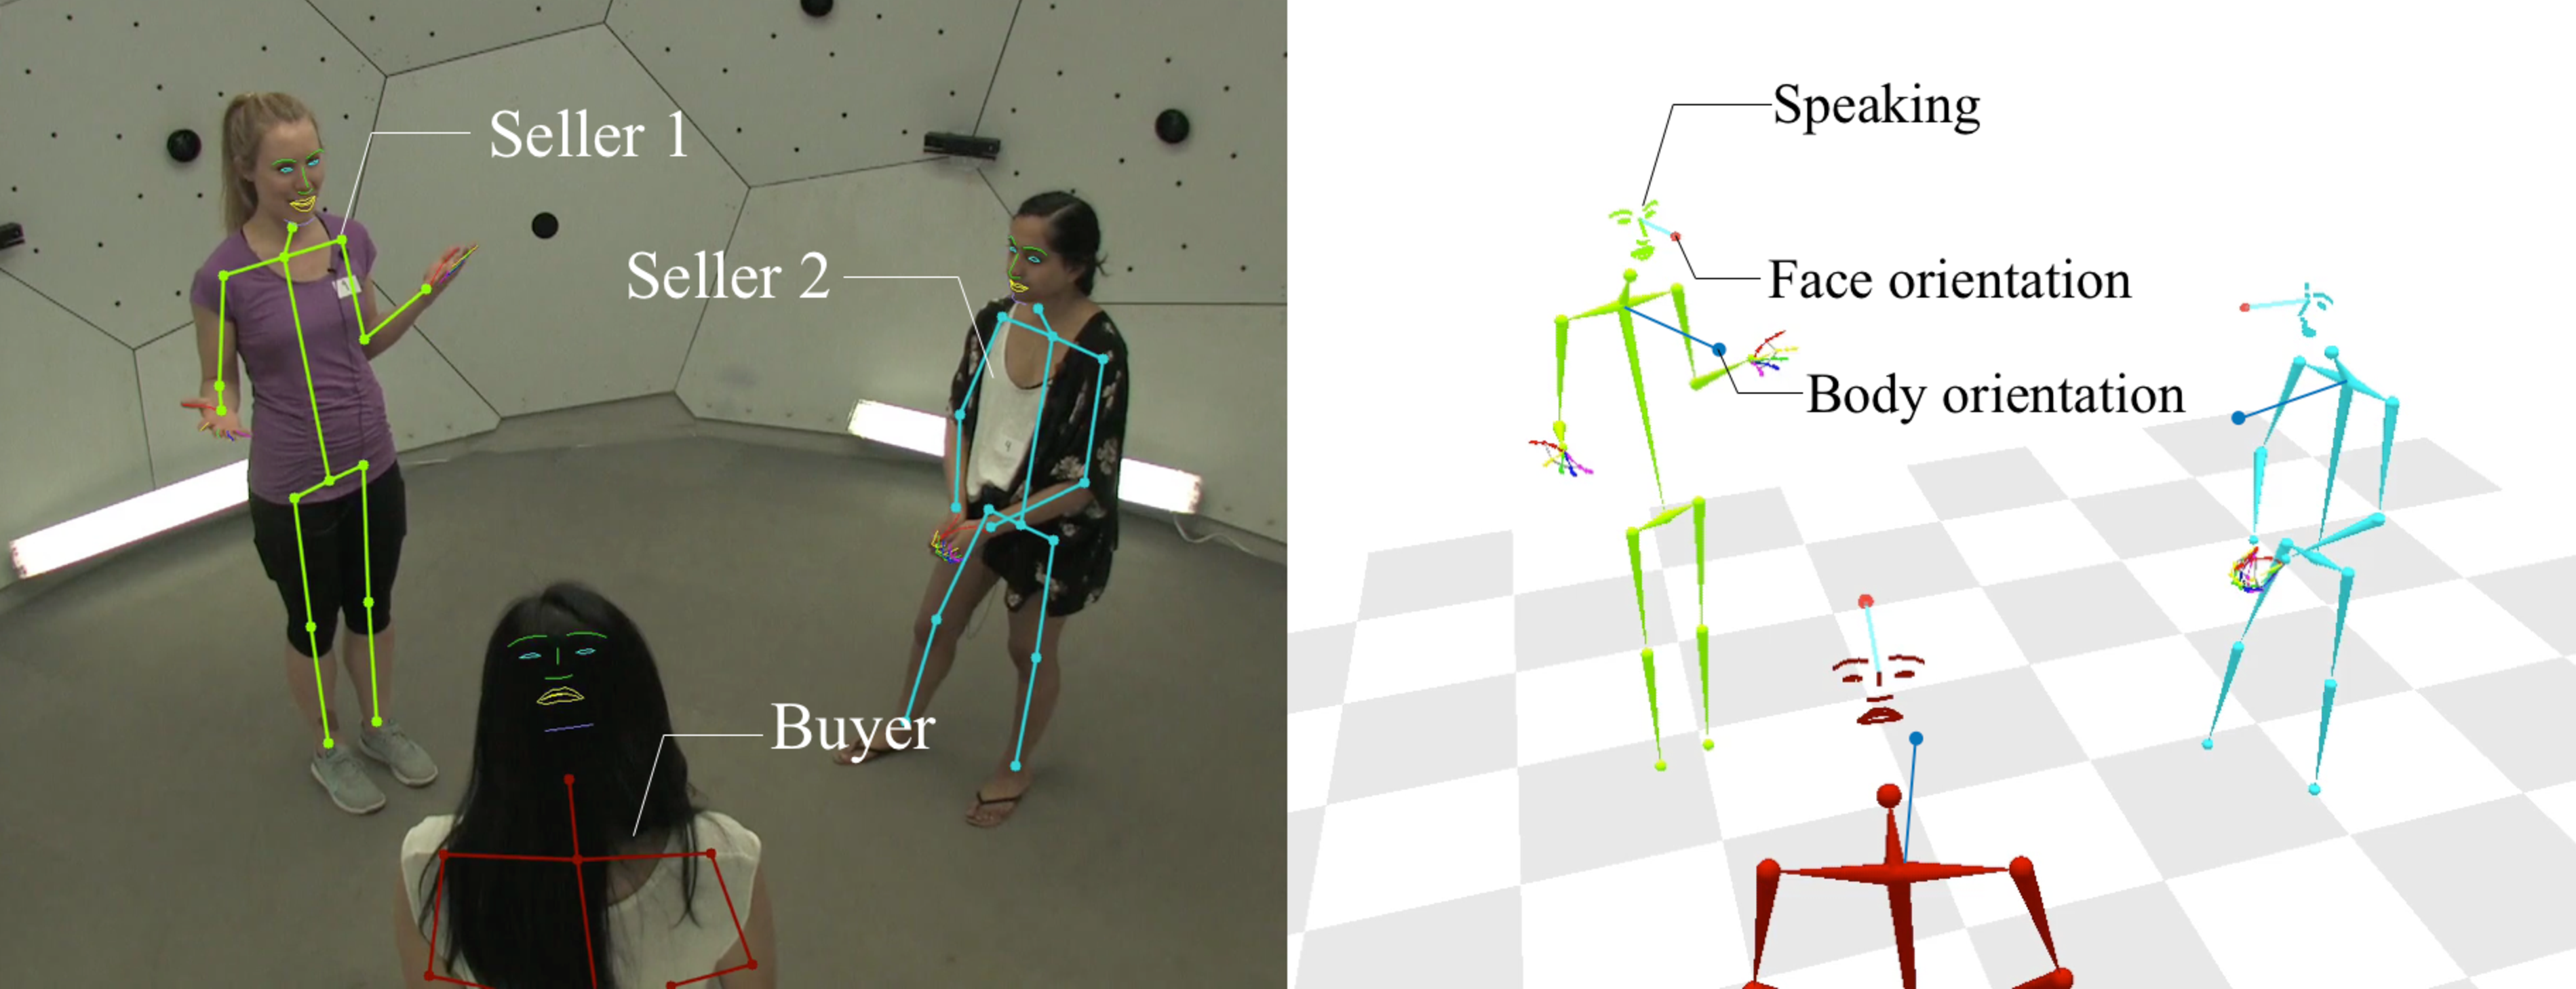
\includegraphics[width=\linewidth]{ssp_fig/haggling_ex}
	\caption{An example of the haggling sequence. (Left) an example scene showing two sellers and one buyer. (Right) Reconstructed 3D social signals showing body, face, and 3D hand motion.} 
	\label{fig:hagglign_ex}
\end{figure}

% We use the state-of-the-art markerless motion capture method to measure the full spectrum of social signals including 3D keypoint from body, face, hands, and foot~\cite{joo2017panoptic, joo2018}. Since this method does not require any sensor attachement on subject's body or other types of initialization asked for the subject during the capture, it can capture natural body behaviors of the interaction. 

\subsection{The Haggling Game Protocol}
To evoke natural interactions, we involved participants in a social game named the \emph{Haggling} game. This game induces a variety of rich non-verbal signals in participants. In our captures, subjects were informed of the rules of the game but were otherwise not instructed about how to behave, nor was their clothing or appearance controlled. They were also not initially aware of our research goals to avoid potential biases in their gestures. The majority of the sequences are captured with people randomly recruited from a university campus. We invent this haggling game to simulate a haggling situation among two sellers and a buyer. The triadic interaction is chosen to include interesting social behaviors such as turn taking, and attention changes, which are missing in dyadic interactions~\cite{rehg2013decoding}. During the game, two sellers are promoting their own comparable products for selling, and a buyer makes the decision about which product he/she buys between the two. They are given a minute for the haggling, and the seller who has sold his/her product is awarded $\$5$. To maximize the influence of each seller's behavior on the buyer's decision-making, the items assigned to sellers are the same type of product with slightly different properties. We provide simple written descriptions to sellers about the items 1 minute before the game. Over the 8 days of captures, 122 subjects participated and 180 haggling sequences were captured (about 3 hours data). The captured sequences contain a lot of voluntary social behaviors of diverse people in a common social context (an example scene is shown in Fig.~\ref{fig:hagglign_ex}. Note that the capture space does not contain other objects which may distract the motion of the target, so we can assume no $X_e(t)$ is necessary in our social signal prediction problem.

\subsection{Measuring Social Signals}
We use the Panoptic Studio System to reconstruct 3D anatomical keypoints of multiple interacting people~\cite{joo2017panoptic, joo2018}. As a key advantage, the method does not require attaching sensors or markers on subject's body, and no behavior restrictions nor initialization poses are needed from the subjects. As output, the system produces 3D body motion $\mathbf{J(t)}$, 3D face motion $\mathbf{F(t)}$, and 3D hand motion $\mathbf{H(t)}$ for each individual at each time $t$. From this measurement, we additionally compute the body orientation $\theta(t)$ and face orientation $\phi(t)$ by finding the 3D normal direction of torso and face. These orientations are computed only on the $x$-$y$ plane with respect to the $y$-axis. We decouple the global location $x$ and body orientation $\theta$ from the body motion capture results, following previous work~\cite{jain2016structural, holden2016deep}, and $\mathbf{J(t)}$ only contains body motions in the person-centric coordinate (root joint is at the origin and body is facing the $z$ direction). An example scene is shown in Fig.~\ref{fig:hagglign_ex}. The voice data $V(t)$ of each individual is also recorded by wireless microphones assigned to each individual. From the audio signal, we manually annotate a binary speaking label $\mathbf{S}(t) \in \{0,1\}$ describing whether the target subject is speaking (labelled as $1$) or not speaking (labelled as $0$) at time $t$. In summary we measure the following signals for each individual:
\begin{equation}
[ \mathbf{x}, \mathbf{\theta}, \mathbf{\phi}, \mathbf{J}, \mathbf{F}, \mathbf{H}, \mathbf{V}, \mathbf{S} ].
\label{equation:measurement}
\end{equation}


% 사람과 같이 행동하는 기계를 만드는 것은 AI와 Robot을 연구하는 모든 사람들의 목표일것이다.  무엇이 사람을 사람답게 만드는가? 특별히 다른 사람들과 의사소통을 하는 능력은 사람을 다른 생물들과 차별시키는 주요한 특징 중에 하나일것이다. 이 논문에서는 인간의 여러가지 특성중 다른 사람과 상호작용하는 능력에 대해 주목한다.  

% 사람과 같이 의사소통을 하는 로봇에 관한 연구는 전혀 새로운것이 아니다. 이미 HCI, HRI, social robotics, AI 등 광범위한 범위에 걸쳐서 이 분야가 연구되고 있다. 하지만 아직까지 실제로 사람과 같이 의사소통을 하는 머신은, 혹은 그렇게 하고 있다고 여겨지는 머신은, 아직 만들어지지 못했다. 그럼 이것이 왜이렇게 어려운 문제이며, 이것을 해결하기 위해서는 어떤 해결책을 모색해야하는걸까?

% 이것을 이야기하기 위해서, 우리는 먼저 "의사소통을" 하는 사람들의 행위에 대해서 다시 한번 생각해볼 필요가 있다. 사람이 의사소통을 한다는것은 과연 무엇일까? 한가지 예를 들어보자. 두명의 사람이 있다. 그 두사람이 대화를 하고 있다고 하자. 우리는 아주 쉽게 이 둘이 대화를 하고 있는지 아닌지를 구분할 수 있다. 이같은 판단을 내릴 수 있는 이유는 무엇인가? 의사소통하지 않는 두명의 모습을 모여줄때랑, 의사소통을 하는 두 사람의 모습을 보여줄때, 한쪽은 커뮤니케이션 중이며, 다른쪽은 아니라는것을 우리는 과연 어떤 기준으로 쉽게 판단할수 있는가? 만일 이것을 쉽게 판단할 수 있는 어떤 규칙을 우리가 발견할수 있다면, 의사소통을 하는 로봇을 만드는 방법은 꽤 간단할 수 있다. 바로 그 규칙을 따르도록 로봇을 만들면 된다. 

% 자, 그럼 이제 의사소통을 하는 사람들의 특징이나 패턴에 대해 한번 생각해보자. 이것또한 새로운 연구주제가 아니다. 이미 아주 오래전부터 pychology 에서 연구되고 고민되는 문제이다. 이 예전 work 들을 들여다보기 전에, 사람의 의사소통이라는게 과연 어떤 목적으로 이루어지는지를 한번 고민해보는게 도움이 될것이다. 

% 사람은 왜 의사소통을 하는가? 바로 서로의 생각과 의견을 주고 받기 위함이다. 우리는 우리 생각을 공유하기 위해 말을 사용하고, 표정을 사용하고, 몸짓, 그리고 모든 미묘한 사람의 몸에서 만들어지는 큐들을 사용한다. 때로는 우리가 굳이 주고받지 않으려고 하는 내용조차도 다른 사람에게 자연스럽게 노출이 되는경우도 있다. 그냥 가만히 무표정하게 서있는다거나, 무의식적으로 몸을 움직인다거나, 그러니까 우리가 의도하고 보내든 그렇지 않든, 우리는 어떠한 형태의 "시그널"을 다른 사람에게 보내고 이 "시그널"은 다른 사람에게 어떤 형태의 메세지를 전달한다. 이 메세지는 언어로 설명할수 있는 레벨이 있을수 있고, 언어를 초월하는 어떤 느낌이나 의도 등의 것들일 수 도있다. 한편으로는 사람의 커뮤니케이션은 기계들의 커뮤니케이션과 유사하다. 이 커뮤니케이션 형태를 통해 어떤 정보가 교환된다. 한가지 큰 차이점은, 기계의 커뮤니케이션에서는 통신을 위한 프로토콜 (이를테면 데이터를 encoding/decoding 하는 규칙) 이 미리 잘 정의되어있지만, 사람의 통신에서는 그것이 아직 명확하게 정의되고 있지는 않다는것이다. 재미있는 사실은, 정의가 되어있지 않을뿐이지 우리가 몸으로 익힌 규칙들은 분명 존재한다. 그리고 대다수의 사람들이 거의 동일한 프로토콜을 유지하고 있다 (성별, 연력, 문화에 따라 다를 수 있다). 단지 이 규칙을 명확하게 정의할수 없기에, 같은 능력을 머신에게 주는것이 어려운 일이 될 뿐이다.  이것을 명확하게 보여주는 한 예가 facial expression이다. 다윈은 이것이 인종과 문화와 독립적으로 어디서나 universal하게 적용된다는 사실에 주목하였다. 그리고 이런 얼굴 표정의 코드를 이해하기 위해, 더 자세하게는, 얼굴의 코드와 인간이 느끼는 감정의 매핑을 정의하고 찾아내기 위한 많은 연구들이 이루어졌다. 

% 하지만 얼굴이 아닌 다른 부분을 생각한다면 굉장히 어려워진다. 가령 사람의 미묘한 손이나 몸의 움직임또한 대화에서 중요한 무언가를 의미할수 있다. 그리고 이런것들이 사람의 따라 정도의 차이는 있어도 굉장히 쉽게 그 의미가 해석이 될수 있다. 그리고 이런것들은 굉장히 연구가 되지 않은 분야중에 하나이다. 이런느낌은 얼굴에서 흔히 적용되는 categorial 하게 의미를 적용하기도, 또 어떠 디멘션을 주기도 모호하다. 특히 이런 경우는 굉장히 많은 변화와 규칙이 있을수 있기에 그것을 정의하는 방법, 혹은 코딩하는 방법조차 거의 연구가 되지 않고 있는 상황이다.

% 즉 이렇듯 인간 스스로가 사용하는 방법에 대한 명확한 연구나 이해가 되어있지않은 상황에서, 이같은 능력을 기계한테 부여하는것은 굉장히 어려운 문제일것이다. 그럼에도 불구하고, 기계가 진짜 인간과 같아지고, 인간의 세상을 이해하고, 또 인간과 진정한 동료나 동반자로 여겨지게 만들기 위해서는, 반드시 이 분야의 연구의 진전을 만들어내야만 할것이다. 


% 자. 지금까지 내용을 요약해보자. 인간의 의사소통이란 뭔가 상호간에 정보 (메세지, 느낌, 의도)를 주고받는 행위를 의미한다. 그리고 이같은 통신을 위해 이들이 정보를 주고받는 방법, 즉 프로토콜, 이 존재하고, 인간만이 이해하는 어떤 룰에 의해 이정보가 인코딩되고 디코딩 되게 된다. 이 프로토콜은 아직 제대로 measure 되거나 modeling되지 않고 있으며, 이런 난해함은 이것을 기계하게 전송하지 못하게 만드는 한계점을 가지게 된다. 


% 자 이런 상황에서 이제, 과거에는 어떤 시도들이 있었는지 한번 생각해보자. 


% 사람이 의사소통을 할때 보여주는 다양한 특징들이 있다. 

% Proxemics는 가장 명확하게 보이는 특징이다. 의사소통을 할때, 사람이 형성하는 거리 (proxemics)나 formation(F-formation) 에는 눈에 띄는 분명한 기준이 있다. Hall 과 XXX의 이론은 가장 대표적인 이론이다. 이 이론에서 정의하는 룰들은 의사소통을 하지 않는 사람들과 비교해볼때 분명한 차이가 보인다. 길을 걸어가는 사람을 둘러보자. 일정한 간격을 유지하면서 비슷한 속도로 걸어가는 두사람이 있다면 우리는 그들이 일행이라고 쉽게 알아볼 수 있다. 일정한 거리를 두고, 마주보고 서있다면 더 명확해진다. 이것은 그들이 전혀 대화를 하거나 하는 좀 더 명확한 특징을 보여주지 않더라도 분명하다. Dimension의 측면으로도 우리는 위치를 2D 라고 정의할수 있고 (평면위에), orientation을 1d, 혹은 2D로 정의해볼수 있을것이다. 즉 표현하고자 하는 dimension이 작고, 그 분명한 특징때문에, 간단한 사진등에 의한 manual한 분석이 가능해진다. 이런 이론이 잘 맞아 떨어진다면, 우리는 이것을 로봇에 적용할수 있을것이다. 로봇이 사람과 이루는 적당한 거리를 예측하고, 그 방향을 분석한다. (Marynel Vazquez])

% Facial Expression도 어느정도 작용을 한다고 본다. 하지만, 약간 언어를 보완하는 역할정도 한다고 여겨질수도 있다. 가령, 어떤 경우에는 거의 아무런 표정없이 대화가 진행되어도 전혀 어색하지 않은 대화가 있을수도 있다. 

% 바디는 더더욱 그러하다. 바디가 있어서 자연스럽지만, 해석도 어렵고 정의도 힘들다. 하지만 바디 모션이 있고 없고는 분명한 차이가 있을수도 있다. 



% 데이터가 부족하다. 바디는 특히. 

% 실제 대화하는 사람을 촬영한 데이터는 더욱. 왜 없을까?? vision 기술의 한계


% computer vision의 한계를 넘어서 이것을 가능하게 하자가 첫번째 목표. 



% 이 문제를 해결하기 위한 중요한 키워드는 두가지이다. 첫째, 최근에 눈부신 성장을 한 데이터 드리븐 기반 방법이 소셜 커뮤니케이션을 이해하기 위한 프로토콜을 정의하는 한가지 중요한 키워드가 될 수 있다.  둘째, 이 방법은 unsupervised 로 풀어야만 한다. 왜냐하면 인간이 label할 수 있는 영역의 한계가 있기 때문이다. 가장 쉬운 예로 affect recognition의 경우만 보더라도 인간의 감성을 카테고리로 볼지 dimension 으로 볼지의 문제를 차치하더라도, 그것을 레이블 하는것 자체가 subjective할수 밖에 없는 일이다. body의 경우는 그 dimension을 정의하는게 훨신 애매하다. 따라서 label을 하는것 대신에 이를 대체할만한 unsupervised 혹은 self-supervise method 의 접근이 해결책이 될 수 있다. 


% 이 논문에서는 사람의 social

% Proxemics F-formation
% Future motion prediction (social force)

% \section{Necessity of New Dataset}

% non-instructed, non exagerated motion
% in a natural discussion scenario

% Full body motion (face + body + hand)

% More than two people. 

% No orientation constraint

% Should be natural. Rich enought. 